\subsection{Fetch application settings}\label{subsection:applied-methods:prototypical-implementation
:load-remote-settings}

The application shell uses Dynamic Module Federation. The \ac{URL} of a micro-frontend is fetched and stored at the startup process of the application shell. The problem with static Module Federation is that the \ac{URL} of the remote application must be known at build time. However, this is troublesome if the application should be built once and deployed to multiple stages, like staging, testing and production. It is very tedious to build the same artifact for every environment. The location of micro-frontends in the cluster may change from time to time, requiring the artifacts to be recreated.

\bigskip

\noindent One possibility to fetch the remote definitions at startup is to store them in a simple \ac{JSON} file, which can be configured for every environment. The application shell makes a GET request to get the configuration from the \ac{JSON} file. The file is provided alongside the application and can be accessed via the same \ac{URL}. The content of the file is a simple mapping between the name of the remote and their location, as shown in Listing \ref{code:applied-methods:define-module-federation-manifest}.

\ifshowListings
\begin{listing}[H]
\begin{minted}{json}
{
  "sales": "http://localhost:4201",
  "contact": "http://localhost:4202",
  "dashboard": "http://localhost:4203",
  "user": "http://localhost:4204"
}
\end{minted}
\caption{The structure of the micro-frontend configuration file with the name and \ac{URL}.}\label{code:applied-methods:define-module-federation-manifest}
\end{listing}
\fi

\noindent The application shell must retrieve the configuration at startup. The configuration is stored inside a map, as shown in Listing \ref{code:applied-methods:load-module-federation-settings}. If the file can be fetched successfully, the application's bootstrap file is imported and run dynamically.

\ifshowListings
\begin{listing}[H]
\begin{minted}{typescript}
fetch('/assets/module-federation.manifest.json')
  .then((res) => res.json())
  .then((definitions) => setRemoteDefinitions(definitions))
  .then(() => import('./bootstrap').catch((err) => console.error(err)));
\end{minted}
\caption{Load the micro-frontend definition file during initialization.}\label{code:applied-methods:load-module-federation-settings}
\end{listing}
\fi

\noindent Another use case for dynamic settings is the configuration of a micro-frontend. This configuration includes the endpoint of the GraphQL \ac{API}, which can be different in staging and production. Therefore, this configuration should also be retrieved dynamically at startup. The settings are retrieved when the application is loaded for the first time and stored for later use. The settings are stored inside a file called \texttt{settings.json}, served alongside the application. Angular provides a handy mechanism in the form of the \texttt{APP\_INITIALIZER} injection token to run initialization logic when the application is loaded.

\bigskip

\noindent The injection token \texttt{APP\_INITIALIZER} enables execution of asynchronous code at application startup. These tasks include retrieving data from a remote \ac{API} and setting up configuration or initializing third-party libraries. When an Angular application loads, it executes all functions registered with \texttt{APP\_INITIALIZER} in the order in which they were defined. If any of the initialization tasks fail, the application will not load. \cite{misc:-:applied-methods:prototype-implementation:angular-app-initializer}

\bigskip

\noindent Listing \ref{code:applied-methods:fetch-and-store-settings} shows a simplified version for fetching and storing the settings in local memory. The settings are fetched from the \texttt{settings.json} file, which content is used to configure the application. The settings of the application shell are stored with the key \texttt{host}. Each application of the micro-frontend architecture has this function, which stores its settings with its unique application name as the key. This is done to retrieve the settings that are used later when configuring the Apollo Client. 

\ifshowListings
\begin{listing}[H]
\begin{minted}{typescript}
@NgModule({
  providers: [{
    provide: APP_INITIALIZER,
    async useFactory(http: HttpClient, storage: StorageClient) {
      const environmentConfig = await lastValueFrom(
        http.get('assets/settings.json')
      );
      storage.store('host', environmentConfig);
    },
    multi: true,
    deps: [HttpClient, StorageClient],
  }]
})
class CoreModule {}
\end{minted}
\caption{Fetch \& store the settings of the application shell.}\label{code:applied-methods:fetch-and-store-settings}
\end{listing}
\fi

\subsubsection{Fetching the settings of the micro-frontends}\label{subsubsection:applied-methods:prototypical-implementation
:load-the-configuration}

Each application of the prototypical micro-frontend architecture follows this approach. When an application is initialized, the application configuration is taken from the file \texttt{settings.json}. As mentioned in the previous section, each micro-frontend stores its settings with the application name as the key when running in standalone mode. However, the configuration is not retrieved if the application shell uses the functionality of a micro-frontend via Module Federation. Therefore, the application gives errors because it cannot access its settings from the storage service. To solve the problem of missing settings for the application, the configuration of a remote application is retrieved and stored in memory when the user activates the route to it. This process is shown visually in Figure \ref{fig:applied-methods:load-remote-settings}.

\ifshowImages
  \begin{figure}[H]
  \centering
  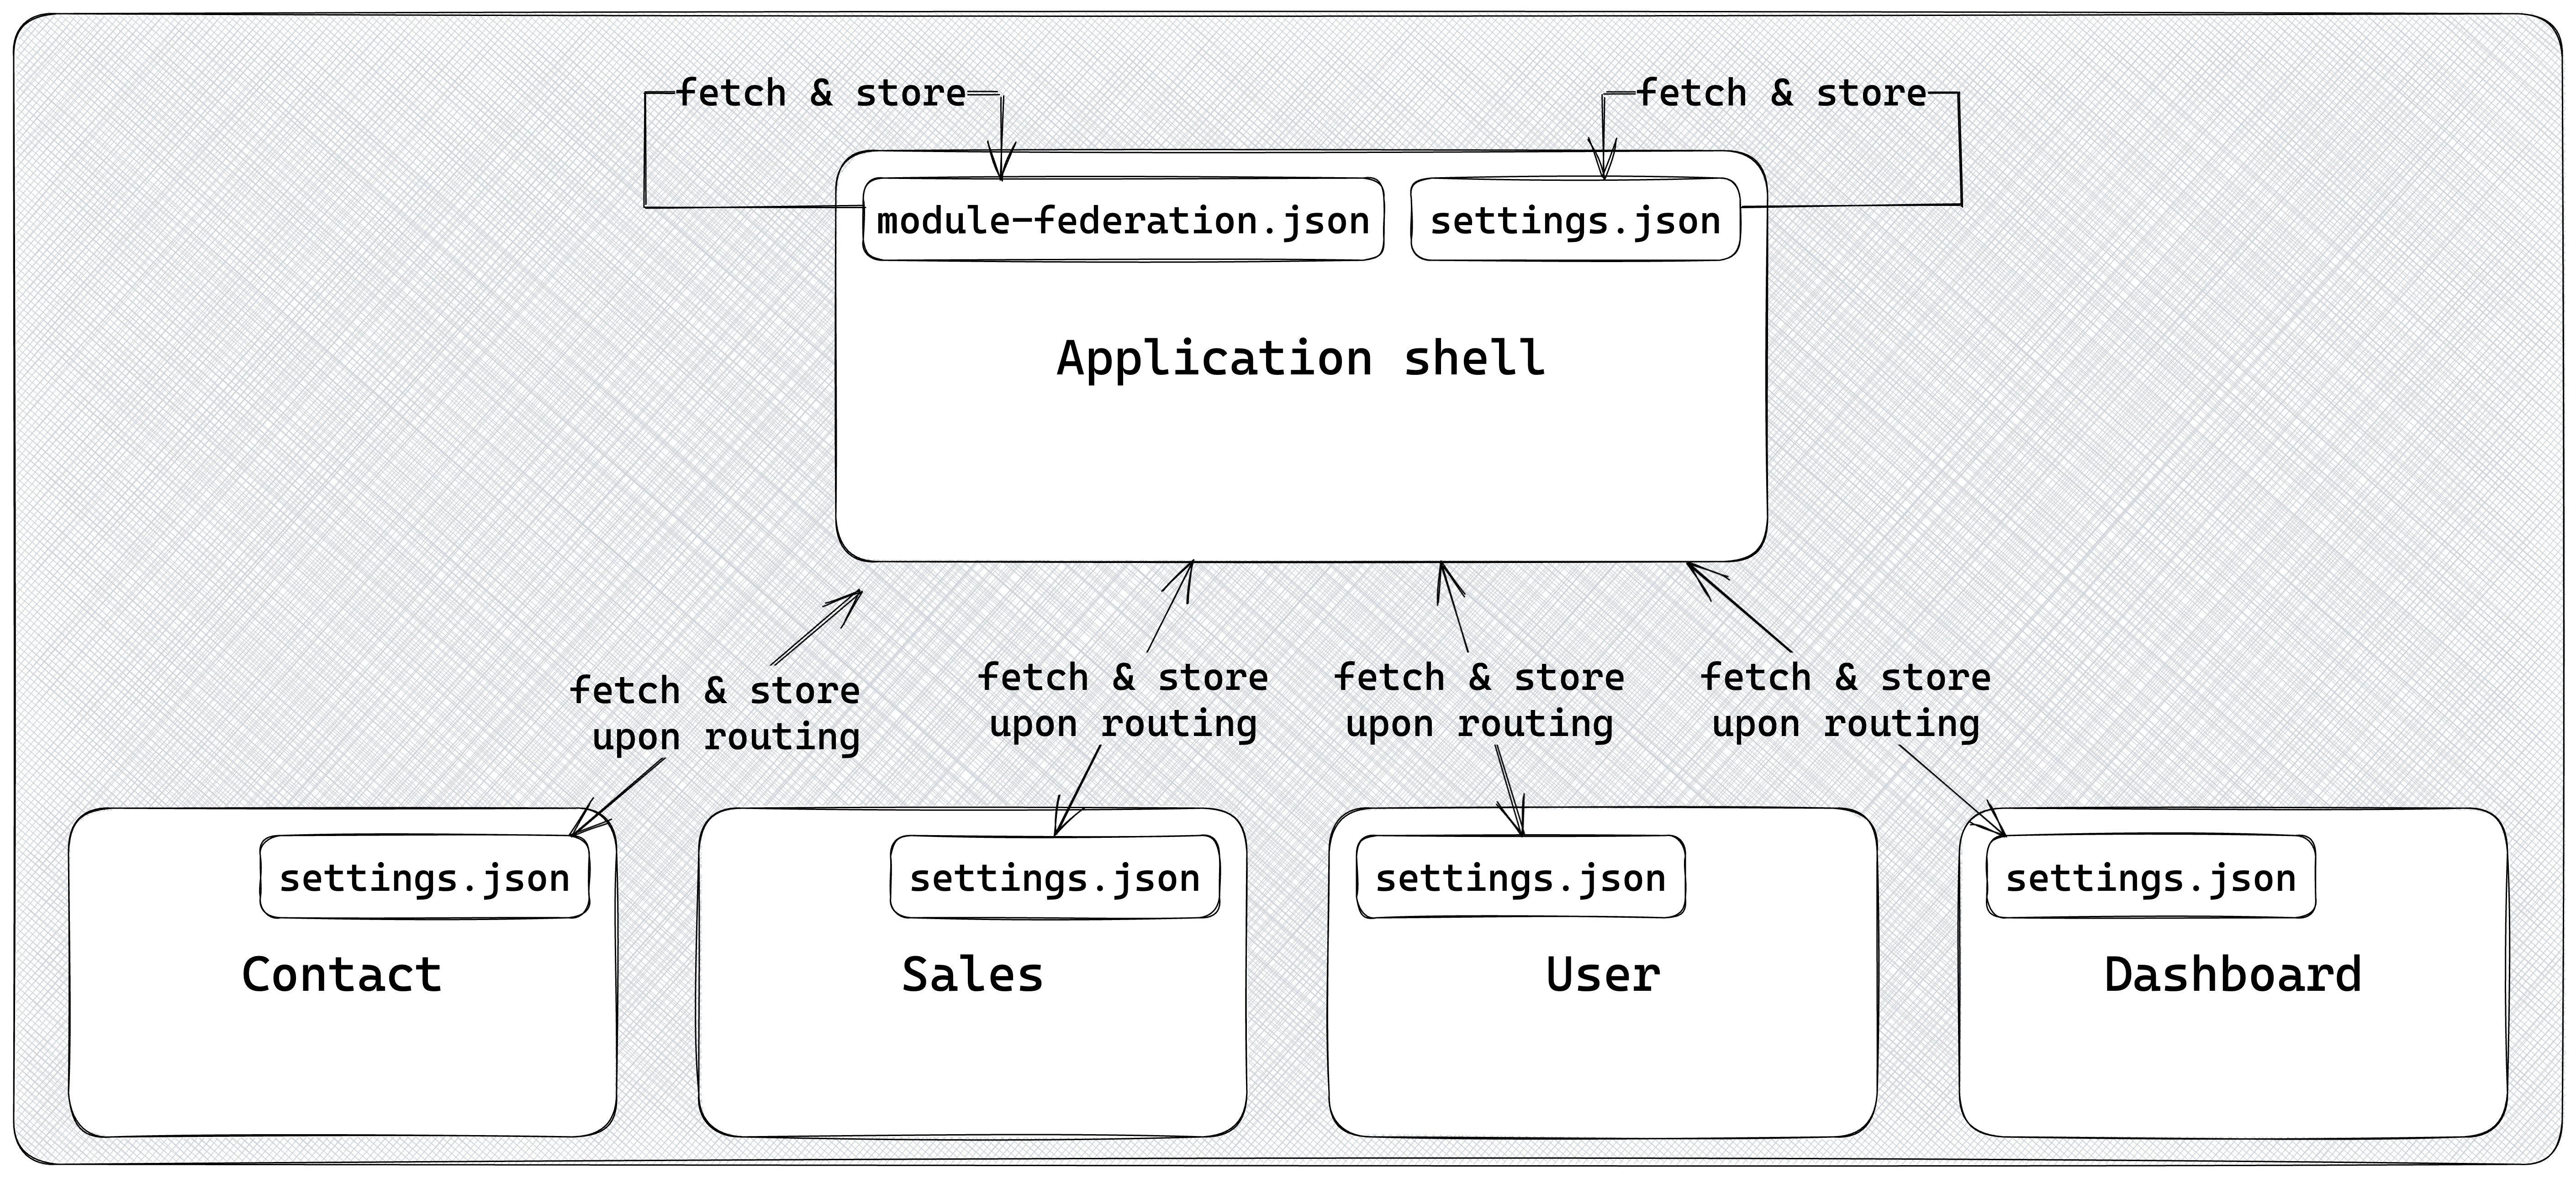
\includegraphics[width=1\linewidth]{images/applied-methods/prototypical-implementation/load-remote-settings.png}
  \caption{Fetch \& store the configuration of the micro-frontends.}\label{fig:applied-methods:load-remote-settings}
  \end{figure}
\fi

\noindent The Angular router provides a handy tool to execute code when a route is activated. This tool is called \texttt{resolver}. A resolver is a service that is executed before the component is rendered. The resolver can be used to fetch data from a remote \ac{API} and make it available to the component. \cite{misc:-:applied-methods:micro-frontends:angular-router-resolver} The \acp{URL} of the micro-frontends are known because they were fetched when the application shell initialized. Therefore the micro-frontend location can be used to fetch and store the \texttt{settings.json} in addition to fetching and rendering the remote module. A simplified version of the code to fetch and store the settings of a micro-frontend is shown in Listing \ref{code:applied-methods:fetch-and-store-remote-application-settings}. The same principle applies to every remote module inside the architecture.

\ifshowListings
\begin{listing}[H]
\begin{minted}[escapeinside=||]{typescript}
const routes: Routes = [{
  path: 'contact',
  loadChildren: () => loadRemoteModule('contact', './Module')
    .then((m) => m.ContactRemoteEntryModule),
  resolve: {
    settings: () => {
      const contactUrl = inject(StorageClient).get('manifest')['contact'];
      return inject(HttpClient).get(contactUrl + '/assets/settings.json');
    }
  }
}]
\end{minted}
\caption{Fetch \& store the settings of the contact micro-frontend.}\label{code:applied-methods:fetch-and-store-remote-application-settings}
\end{listing}
\fi

\noindent This pattern of retrieving settings allows each consumed micro-frontend to access its settings in the same way as when it is running in standalone mode. Another advantage is that each application accesses its own settings and not the settings of the other applications. 
